\documentclass[10pt,a4paper]{article}
\usepackage{fontspec}
\setmainfont{Times New Roman}
\usepackage[russian,english]{babel}
\usepackage[margin=2cm]{geometry}
\usepackage{amsmath,amssymb,graphicx,longtable,array,booktabs}
\usepackage[numbers,sort&compress]{natbib}
\usepackage[unicode,hidelinks]{hyperref}
\usepackage{url}
\Urlmuskip=0mu plus 2mu
\usepackage{titlesec}
\titleformat{\section}{\normalfont\bfseries\fontsize{10}{12}\selectfont}{}{0pt}{}
\titleformat{\subsection}{\normalfont\bfseries\fontsize{10}{12}\selectfont}{}{0pt}{}
\titlespacing*{\section}{0pt}{7pt}{3pt}
\titlespacing*{\subsection}{0pt}{5pt}{2pt}
\setlength{\parindent}{1.25cm}
\setlength{\parskip}{0pt}
\setlength{\emergencystretch}{3em}
\pagestyle{empty}
\begin{document}
\selectlanguage{russian}
\noindent УДК [УТОЧНИТЬ АВТОРОМ: рекомендуемая область 004.8]\par
\noindent [ФАМИЛИЯ И. О. АВТОРА 1], [ФАМИЛИЯ И. О. СОАВТОРА ПРИ НАЛИЧИИ]\par
\noindent [ПОЛНОЕ НАЗВАНИЕ ОРГАНИЗАЦИИ], [ГОРОД], [СТРАНА]\par
\begin{center}\bfseries Контроль достижимости параметрической компрессии при локальном структурном прунинге графовых нейронных сетей без дообучения\end{center}
\noindent Аннотация. Рассматривается локальное структурное удаление скрытых каналов графовых нейронных сетей без дообучения. Цель работы — отделить влияние механизма соблюдения целевой параметрической компрессии от влияния обучаемой стратегии выбора действий и показать роль распределения ширин между слоями. Предложен и исследован технический механизм фильтрации действий по точной достижимости целевого диапазона с учётом целочисленного числа параметров и оставшегося горизонта. Механизм не использует метки классов и применяется одинаково к табличному Q-learning, жадной стратегии и случайному выбору действий. Пилотное исследование основано на ранее полученных результатах для Cora и трёхслойных GCN и GraphSAGE с двумя скрытыми слоями ширины 32. Для каждой архитектуры использован один замороженный обученный checkpoint; три повторения относятся к генератору случайных чисел политики, а не к независимым обучениям сети. При целях 30 и 50 \% и допуске $\pm$1 процентный пункт каждая из трёх ограниченных стратегий попала в диапазон во всех 12 локальных оценках. Жадная стратегия имела не меньшую среднюю валидационную accuracy, чем Q-learning, во всех четырёх условиях и требовала меньше поиска. Анализ 80 ранее сохранённых случайных масок обнаружил существенную вариативность как между ширинами, так и при фиксированных ширинах. В 34 парных исполнениях на локальном CPU и POWER8 совпали действия, сохраняемые каналы и тензоры итоговых моделей. Результаты подтверждают полезность явного контроля допустимости, но не устанавливают преимущество обучения с подкреплением, качество на тестовой выборке или ускорение инференса. Выводы ограничены одним графом и одним обученным checkpoint на архитектуру; новых научных экспериментов при подготовке статьи не проводилось.\par
\noindent Ключевые слова: графовые нейронные сети; структурный прунинг; удаление каналов; параметрическая компрессия; достижимость; Q-learning; воспроизводимость\par
\noindent [SURNAME I. O. OF AUTHOR 1], [SURNAME I. O. OF COAUTHOR IF APPLICABLE]\par
\noindent [FULL OFFICIAL AFFILIATION], [CITY], [COUNTRY]\par
\begin{center}\bfseries Reachability control of parameter compression in local structural pruning of graph neural networks without fine tuning\end{center}
\noindent Abstract. This study examines local structural pruning of hidden channels in graph neural networks without fine tuning. The objective is to separate explicit control of target parameter compression from the contribution of a learned action selection policy and to examine how layer width allocation affects the observed results. A technical mechanism filters actions using exact reachability of the target band under integer parameter counts and a remaining action horizon. The filter requires no class labels and is shared by tabular Q-learning, greedy selection, and random action selection. The pilot study reanalyses existing Cora results for three-layer GCN and GraphSAGE models with two hidden layers of width 32. Each architecture has one frozen trained checkpoint. Three repetitions vary the policy random number generator rather than the network training seed. At compression targets of 30 and 50 percent with a tolerance of one percentage point, each constrained strategy reached the band in all 12 local evaluations. Greedy selection achieved validation accuracy at least as high as the mean Q-learning accuracy in all four model and target conditions, while requiring less search. An additional analysis of 80 archived random masks shows substantial variability both across width configurations and within identical configurations. Across 34 paired local CPU and POWER8 executions, selected actions, retained channel identities, and final checkpoint tensors matched. These results support explicit feasibility control but do not establish reinforcement learning superiority, test set performance, or inference acceleration. The evidence is limited to one graph and one trained checkpoint per architecture.\par
\noindent Keywords: graph neural networks; structural pruning; channel removal; parameter compression; reachability; Q-learning; reproducibility\par
\clearpage
\section*{Введение}
Графовые нейронные сети используются для обработки связанных объектов, когда предсказание зависит одновременно от признаков вершины и её окружения. Архитектуры GCN и GraphSAGE представляют два распространённых подхода к построению таких представлений \cite{r1,r2}. Для их компактного развёртывания можно уменьшать размерности скрытых представлений. При структурном прунинге удаление канала сопровождается физическим уменьшением связанных матриц; число параметров действительно сокращается. Такой подход связан с общим направлением сжатия сетей посредством удаления каналов, в частности Network Slimming \cite{r3}. При этом уменьшение числа параметров и уменьшение времени выполнения являются разными результатами.\footnote{GNN: graph neural network; GCN: graph convolutional network; GraphSAGE: graph sample and aggregate; CPU: central processing unit; SD: sample standard deviation; DP: dynamic programming; PyG: PyTorch Geometric.}

В многослойной сети одинаковая доля удалённых каналов в разных слоях даёт неодинаковую параметрическую компрессию. Более того, близкое итоговое число параметров совместимо с существенно различными скрытыми ширинами. Поэтому сравнение только по запрошенному проценту прунинга смешивает по меньшей мере три фактора: соблюдение цели, распределение ширин и выбор конкретных сохраняемых каналов. Для адаптивного метода добавляется правило остановки. Если оно не контролирует достижимость цели, алгоритм может пройти через допустимый диапазон и завершиться далеко за его пределами.

Настоящая работа рассматривает этот вопрос на завершённом пилотном наборе результатов. Объект исследования — физическое локальное удаление каналов уже обученных трёхслойных GCN и mean GraphSAGE без дообучения. Цель исследования — установить, какую часть наблюдаемого поведения объясняет явный контроль достижимости целевой компрессии и есть ли в этих условиях дополнительная польза табличного Q-learning относительно простых стратегий с теми же операциями. Для этого анализируются ранее выполненные варианты остановки и три стратегии с общим фильтром допустимости. Дополнительные результаты характеризуют разброс случайных масок и парную воспроизводимость исполнения на двух CPU-платформах.

Вклад работы состоит в реализации точного фильтра достижимости для рассматриваемого пространства локальных удалений, формулировке условий его гарантии и контролируемом анализе уже полученных результатов. Само динамическое программирование, структурный прунинг и Q-learning не заявляются новыми. Приоритет на общий принцип ограничения действий по достижимости не устанавливается. Техническое решение рассматривается как собственная реализация механизма в данном протоколе, а не как доказанно новый универсальный алгоритм. Эмпирический вывод также узок: соблюдение параметрической цели обеспечивается фильтром, тогда как преимущества обучаемой политики перед жадным контролем в данном пилоте не обнаружено.

\section*{Предшествующие исследования}
Гипотеза лотерейного билета связывает успешное разреживание с существованием обучаемых подсетей и их инициализацией \cite{r4}. В работе Unified GNN Sparsification этот подход перенесён на совместное разреживание матрицы смежности и весов GNN \cite{r5}. Направление Graph Sparse Training, представленное в 2024 г., изменяет разреженность на уровне графовых данных, сохраняя семантическую и топологическую информацию \cite{r6}. В исследовании 2025 г. Pruning for GNNs анализируются избыточные структуры механизмов распространения сообщений и выразительность получаемых архитектур \cite{r7}. Эти работы подтверждают разнообразие постановок прунинга GNN. В настоящей статье граф, вершины, рёбра и размерность входных признаков фиксированы: удаляются только скрытые каналы модели. Поэтому опубликованные результаты разреживания графа не являются численными baseline для наших таблиц.

SNIP оценивает чувствительность связей перед обучением, а GraSP ориентирован на сохранение потока градиента при прунинге инициализированной сети \cite{r8,r9}. Использование производных этих критериев после обучения и их агрегация по целым каналам меняют постановку. В архиве проекта имеются функциональные проверки соответствующих постобучающих адаптаций, однако их короткий диагностический режим не включён в основное сравнение статьи. Такой выбор предотвращает смешение проверки работоспособности с исследованием сравнительного качества. Основные контролируемые стратегии используют один и тот же текущий magnitude-критерий выбора каналов, поэтому различаются прежде всего выбором действий и правилом допустимости.

Обучение с подкреплением применялось для автоматического выбора политики сжатия в AMC \cite{r10}. Однако эта работа исследует иной класс моделей и другое пространство управления. Её результаты не позволяют заранее ожидать преимущества табличной политики в небольшом дискретном пространстве GNN. Исследование Rethinking the Value of Network Pruning подчёркивает необходимость различать найденную архитектуру и унаследованные параметры \cite{r11}. В нашем режиме веса не переобучаются, поэтому идентичность каналов остаётся самостоятельным источником вариативности. Работы по оценке GNN показывают чувствительность выводов к разбиениям данных и процедуре обучения \cite{r12}. Соответственно, повторения политики на одном checkpoint здесь не интерпретируются как повторные независимые обучения сети.

\section*{Математическая постановка}
Пусть задан граф G = (V, E), матрица признаков X и фиксированное разбиение вершин на обучающую, валидационную и тестовую части. Исходная сеть M$_0$ уже обучена. Во время анализируемого поиска используются только валидационные метки. Для трёхслойной модели размерности имеют вид F $\to$ a $\to$ b $\to$ C, где F и C фиксированы, а a и b обозначают текущие скрытые ширины. Исходные ширины равны 32; минимальная ширина каждого скрытого слоя равна 4.

Для поддерживаемого GCN с bias каждого слоя число параметров определяется формулой

\begin{equation}
P_{\mathrm{GCN}}(a,b)=Fa+ab+bC+a+b+C.
\end{equation}
В mean GraphSAGE используются две матрицы весов на слой, для соседнего представления и корневой вершины; bias присутствует только в одной ветви. При root\_weight=True, project=False и normalize=False получаем

\begin{equation}
P_{\mathrm{SAGE}}(a,b)=2(Fa+ab+bC)+a+b+C.
\end{equation}
Формулы относятся именно к этим реализациям и не переносятся без проверки на варианты с дополнительными проекциями, нормализацией или другими параметрами. Для Cora F = 1433 и C = 7, поэтому P$_0$ равно 47 175 для GCN и 94 279 для GraphSAGE. Графовые данные и их хранение в это число не входят.

Параметрическая компрессия s и целевое множество B определяются следующим образом:

\begin{equation}
s(a,b)=1-\frac{P(a,b)}{P_0}.
\end{equation}
\begin{equation}
B=\{(a,b)\in\mathbb{Z}^2:4\leq a,b\leq32,\ |s(a,b)-s^*|\leq\tau\}.
\end{equation}
Здесь s* $\in$ \{0,30; 0,50\}, $\tau$ = 0,01. Допуск означает $\pm$1 процентный пункт, а не относительный один процент от цели. Число удалённых каналов является другой характеристикой. Попадание в цель проверяется по фактическому целому числу параметров, до округления процентов для таблицы.

Локальное действие u = ($\ell$, k) удаляет k $\in$ \{1, 2, 4, 8\} каналов скрытого слоя $\ell$ $\in$ \{0, 1\}. После действия ширина не может стать меньше 4. Можно возвращаться к ранее обработанному слою; порядок обхода не фиксирован. При выборе каналов суммируются модули связанных входящих и исходящих весов и скрытого bias в текущей модели. Удаляются каналы с наименьшей суммой; равенства разрешаются по текущему индексу. Соответствующие строки выбранного слоя и столбцы следующего слоя физически исключаются, включая обе весовые ветви GraphSAGE. Сохраняются исходные идентификаторы каналов, позволяющие проверить проекцию итоговых тензоров из M$_0$. Структурное уменьшение не означает удаления вершин или рёбер.

\section*{Метод контроля достижимости}
Введём d(n), минимальное число допустимых удалений для суммарного сокращения ширины на n каналов. Для неотрицательного целого n используется конечная рекурсия

\begin{equation}
d(0)=0,\qquad d(n)=1+\min_{k\in\{1,2,4,8\},\ k\leq n}d(n-k),\quad n>0.
\end{equation}
Из текущих ширин (a, b) при оставшемся горизонте h целевая пара (x, y) достижима тогда и только тогда, когда x $\leq$ a, y $\leq$ b и d(a $-$ x) + d(b $-$ y) $\leq$ h. Действие сохраняется в допустимом множестве, если после его применения остаётся хотя бы одна такая пара из B с горизонтом h $-$ 1. Множество B перечисляется по целым ширинам; сравнение компрессии с целью выполняется рациональной арифметикой. Для исходных ширин 32 проверяется не более 841 пары. Метки классов, accuracy и значения Q при этом не используются.

Гарантия относится к параметрической достижимости. Если начальное B достижимо за заданный горизонт, все действия уменьшают ровно одну ширину на допустимое k, минимум ширины неизменен, фильтр применяется перед каждым выбором, а вне B нельзя остановиться, то любая разрешённая последовательность достигает B не позднее исчерпания горизонта. Действительно, выбранное действие сохраняет достижимое продолжение. До попадания в B такое продолжение содержит хотя бы один шаг, следовательно, множество разрешённых действий непусто. После каждого удаления h уменьшается на один. При h = 0 достижима только текущая пара, которая поэтому должна принадлежать B. Монотонность ширин гарантирует допустимость промежуточных значений. Это доказательство не использует качество выбранных каналов.

Если начальная цель недостижима, реализация завершает процедуру с событием initial\_target\_infeasible, не расширяя допуск. При достижении B поиск автоматически заканчивается; off-band STOP исключён. В реализации приоритеты max\_steps и no\_valid\_actions проверяются до нового события target\_band. Поэтому итоговый флаг попадания вычисляется отдельно: даже при ином терминальном имени фактическая архитектура может принадлежать B. Гарантия не означает оптимальности маски, сохранения accuracy или гарантированного ускорения. Она также не распространяется на дополнительные ограничения качества, не включённые в проверку достижимости.

Три ограниченные стратегии используют одинаковый фильтр. Constrained Random равномерно выбирает разрешённое действие, но конкретные каналы по-прежнему определяются magnitude-критерием. Это не равномерный выбор конечной архитектуры и не случайный выбор каналов. Constrained Greedy оценивает все разрешённые действия и выбирает максимальную немедленную награду с возможным терминальным штрафом; равенства разрешаются порядком действий. Constrained Q использует табличную оценку действий. Тем самым фильтр одинаков, но политика обхода и вычислительная стоимость различаются.

Немедленная награда за успешное удаление и однократно выплачиваемый терминальный штраф имеют вид

\begin{equation}
R_t=0{,}6(s_t-s_{t-1})-0{,}4\max(0,A_0-A_t).
\end{equation}
\begin{equation}
\Phi_T=-\lambda\max(0,|s_T-s^*|-\tau).
\end{equation}
Здесь A$_0$ и A$_t$ — валидационные accuracy как доли единицы, $\lambda$ = 2. За STOP базовая награда равна нулю, затем начисляется терминальный штраф. На последнем удалении к R$_t$ прибавляется $\Phi_t$; штраф не добавляется повторно. Компонента прироста s является показателем сокращения параметров, а не измеренным временем инференса. Штраф за потерю accuracy сравнивает текущее качество с исходным, а не с предыдущим состоянием, поэтому сумма наград зависит от траектории.

Табличное Q-learning основано на стандартном обновлении оценки действий \cite{r13}:

\begin{equation}
Q(z,u)\leftarrow Q(z,u)+\alpha\left[r+\gamma\max_{v\in\mathcal{A}(z')}Q(z',v)-Q(z,u)\right].
\end{equation}
Для терминального перехода bootstrap равен нулю; r уже содержит единственный терминальный штраф, если он применим. Максимум берётся только по разрешённым следующим действиям. Используются $\alpha$ = 0,1, $\gamma$ = 0,9, $\varepsilon$ = 0,2, 100 эпизодов и не более 20 успешных удалений в эпизоде. Каждый эпизод и финальное применение политики начинаются с M$_0$; при финальном применении $\varepsilon$ = 0. Неизвестные табличные значения в базовом варианте равны нулю. Состояние содержит обе ширины, оставшийся горизонт, целую корзину accuracy с шагом 0,01 и терминальный флаг. Исходные идентификаторы каналов в состояние не входят, поэтому одинаковые состояния могут объединять разные физические модели. Это агрегированное представление не даёт оснований переносить на пилот теорему сходимости Q-learning в точной марковской постановке.

\section*{Дизайн исследования и происхождение данных}
Статья представляет вторичный анализ завершённого пилотного исследования, а не новую экспериментальную кампанию. Основная группа V3 включает Cora с 2708 вершинами, 1433 признаками, семью классами и сохранённым edge\_index из 10 556 направленных записей. Последнее число описывает использованный обработанный тензор, а не универсальное число исходных цитирований Cora. Использован полный граф и исходное замороженное разбиение. Модели реализованы средствами PyTorch Geometric \cite{r14}. Обе архитектуры имеют три слоя и скрытые ширины 32/32, dropout 0,5; при оценке применяется eval-режим. Дообучение, повторное обучение и изменение графа отсутствуют.

Для каждой архитектуры использован один ранее обученный checkpoint с training seed 101, происходящий из архива POLUS. Его байтовая и тензорная идентичность зафиксирована отдельно от seed политики. Исходные валидационные accuracy составляют 89,8336 \% для GCN и 88,3549 \% для GraphSAGE. Локальные policy seeds равны 101, 5001 и 5002. В каждой из четырёх комбинаций модели и цели выполнены восемь вариантов, то есть 96 локальных оценок. Два дополнительных фиксированных probe исключены из статистики выполнения цели. На POLUS повторены 32 оценки при policy seed 101 и два probe, всего 34 парных исполнения.

Помимо constrained Q, Random и Greedy рассмотрены базовый Q R2 и четыре отдельные модификации: точное значение STOP как известного терминального штрафа; консервативная инициализация неизвестных Q; случайное разрешение точных равенств максимальных Q; пороговое завершение после первого пересечения s $\geq$ s* $-$ $\tau$. Эти варианты изменяют разные части исходного алгоритма и не комбинируются. Для консервативной инициализации использована нижняя оценка оставшейся суммы наград: $-$0,4 $\sum_{j=0}^{h-1}\gamma^j$ $-$ $\lambda$ max(0, max(s*, 1 $-$ s*) $-$ $\tau$). Она ограничивает неизвестные значения, но не обрезает уже обученные. Пороговая остановка не эквивалентна точному фильтру: одно действие способно перескочить верхнюю границу.

Дополнительная группа V2 содержит по 20 случайных масок на каждую комбинацию модели и цели, всего 80. В ней равномерно выбирается допустимая конечная пара ширин, затем равномерные подмножества каналов заданных размеров. Seeds масок 1000–1019 повторяются между условиями. Эти наблюдения характеризуют вариативность маски на фиксированных checkpoint и разбиении, а не вариативность обученных GNN. Эта группа используется для анализа ширин и каналов; её Random нельзя смешивать с Random действий в V3 или считать ещё 80 независимыми обучениями.

Историческая группа V1 включает Cora, CiteSeer и PubMed, GCN и GraphSAGE и training seeds 101/202/303. В ней отличаются surgery, награда и допуски цели. Поэтому её 252 результата и отдельные исторические исполнения POLUS не входят в численные таблицы этой статьи и не трактуются как абляция V2/V3. Короткая функциональная матрица V2 из 24 комбинаций также не используется для выбора победителя. В частности, исторический Adaptive Greedy при цели 30 \% достигал 31,0758 \% для GCN и 31,0886 \% для GraphSAGE: оба значения строго за верхней границей 31 \%. Терминальное имя target\_reached не заменяет численной проверки допуска.

В сохранённой проверке V3 подтверждены 98 локальных и 34 POLUS физических checkpoint, 9600 эпизодов Q-learning, 110 830 переходов и 75 467 табличных записей. Проверялись проекция весов по сохранённым идентификаторам, строгая загрузка, число параметров, финальные валидационные метрики, арифметика наград и воспроизведение обновлений Q. Эта проверка использовала сохранённые валидационные значения промежуточных состояний; все промежуточные forward заново не выполнялись. При подготовке статьи выполнена только проверка файлов и независимый пересчёт таблиц из CSV: модели не загружались и научные запуски не выполнялись.

В V3 все метки за пределами валидационной части заменены на $-$1 перед адаптивным поиском. Test metrics не вычислялись. Это сохраняет разделение тестовых меток, но не превращает валидационное качество в независимую итоговую оценку: та же валидационная часть входит в награду, жадный выбор и диагностический анализ. Набор следует считать development/pilot. Все последующие сравнения accuracy и macro-F1 относятся только к валидационной части.

\section*{Результаты}
\subsection*{Соблюдение целевой компрессии}
Таблица 1 показывает число попаданий в точный диапазон среди 12 локальных оценок каждого варианта. Базовый Q и отдельные изменения STOP, неизвестных значений Q и разрешения равенств не обеспечили выполнения цели. Базовый Q завершался при компрессии 83,9392–87,7067 \% вместо запрошенных 30 или 50 \%. Пороговая остановка обеспечила все шесть попаданий при цели 50 \%, но при цели 30 \% достигнуто 31,0758–31,3386 \%, то есть верхняя граница была превышена. Constrained Q, Random и Greedy дали по 12/12 попаданий. Это согласуется с инвариантом фильтра и не является свидетельством успешного обучения политики.

\par\medskip\noindent Таблица 1. Выполнение параметрической цели в V3 на локальном CPU\par
\begingroup\setlength{\tabcolsep}{2pt}\renewcommand{\arraystretch}{1.12}
\begin{longtable}{p{0.387\linewidth}p{0.182\linewidth}p{0.182\linewidth}p{0.188\linewidth}}
\toprule
Вариант & Цель 30 \% & Цель 50 \% & Всего\\ \midrule\endhead
Q R2 & 0/6 & 0/6 & 0/12\\
Q точный STOP & 0/6 & 0/6 & 0/12\\
Q консервативный & 0/6 & 0/6 & 0/12\\
Q случайные равенства & 0/6 & 0/6 & 0/12\\
Q пороговая остановка & 0/6 & 6/6 & 6/12\\
Constrained Q & 6/6 & 6/6 & 12/12\\
Constrained Random & 6/6 & 6/6 & 12/12\\
Constrained Greedy & 6/6 & 6/6 & 12/12\\
\bottomrule\end{longtable}\endgroup
Три значения policy seed разделяют один checkpoint на архитектуру. Совпадающие результаты детерминированного Greedy не являются независимыми репликациями. Неопределённость вероятности успешного попадания на других checkpoint из этих долей не оценивается.

\subsection*{Контролируемое сравнение стратегий}
Таблица 2 содержит результаты трёх стратегий с общей проверкой достижимости. Среднее и выборочное стандартное отклонение характеризуют только три policy seed; SD accuracy выражено в процентных пунктах. Для Greedy приведены совпадающие значения без представления их как трёх независимых наблюдений. Точные конечные ширины и числа параметров для всех policy seed приложены к статье в verified\_v3\_results.csv; здесь они также показаны для непосредственной проверки диапазона.

\par\medskip\noindent Таблица 2. Результаты стратегий с фильтром достижимости на одном checkpoint каждой архитектуры\par
\begingroup\setlength{\tabcolsep}{2pt}\renewcommand{\arraystretch}{1.12}
\begin{longtable}{p{0.100\linewidth}p{0.091\linewidth}p{0.170\linewidth}p{0.159\linewidth}p{0.159\linewidth}p{0.159\linewidth}p{0.103\linewidth}}
\toprule
Условие & Метод & Ширины; P & s, \% & Acc., \% & F1, \% & Поиск, с\\ \midrule\endhead
GCN / 30 \% & Q & 23$\times$16; 33 485 / 23$\times$13; 33 392 / 23$\times$15; 33 454 & 29,11 $\pm$ 0,10 & 84,97 $\pm$ 1,89 & 79,74 $\pm$ 4,75 & 11,49\\
GCN / 30 \% & Greedy & 23$\times$16; 33 485 & 29,02 & 86,32 & 83,19 & 0,37\\
GCN / 30 \% & Random & 23$\times$16; 33 485 / 23$\times$11; 33 330 & 29,24 $\pm$ 0,19 & 82,87 $\pm$ 2,99 & 75,93 $\pm$ 6,28 & 0,12\\
GCN / 50 \% & Q & 16$\times$32; 23 719 & 49,72 & 81,33 & 72,81 & 12,16\\
GCN / 50 \% & Greedy & 16$\times$32; 23 719 & 49,72 & 81,33 & 72,81 & 0,21\\
GCN / 50 \% & Random & 16$\times$8; 23 143 / 16$\times$7; 23 119 / 16$\times$18; 23 383 & 50,79 $\pm$ 0,31 & 68,58 $\pm$ 10,73 & 53,10 $\pm$ 15,00 & 0,14\\
SAGE / 30 \% & Q & 23$\times$15; 66 863 / 23$\times$16; 66 924 / 23$\times$12; 66 680 & 29,12 $\pm$ 0,13 & 77,26 $\pm$ 2,06 & 68,28 $\pm$ 4,78 & 65,07\\
SAGE / 30 \% & Greedy & 23$\times$16; 66 924 & 29,01 & 79,48 & 72,87 & 1,50\\
SAGE / 30 \% & Random & 23$\times$16; 66 924 / 23$\times$11; 66 619 & 29,23 $\pm$ 0,19 & 75,17 $\pm$ 3,74 & 64,24 $\pm$ 7,48 & 0,54\\
SAGE / 50 \% & Q & 16$\times$32; 47 383 & 49,74 & 84,84 & 82,49 & 57,78\\
SAGE / 50 \% & Greedy & 16$\times$32; 47 383 & 49,74 & 84,84 & 82,49 & 0,71\\
SAGE / 50 \% & Random & 16$\times$8; 46 255 / 16$\times$7; 46 208 / 16$\times$18; 46 725 & 50,79 $\pm$ 0,30 & 75,91 $\pm$ 7,15 & 64,21 $\pm$ 15,20 & 0,58\\
\bottomrule\end{longtable}\endgroup
Для GCN при цели 30 \% средняя accuracy Q составляет 84,97 \%, Greedy — 86,32 \%, то есть разность Q минус Greedy равна $-$1,36 п.п. Для GraphSAGE соответствующие значения равны 77,26 и 79,48 \%, разность $-$2,22 п.п. При цели 50 \% accuracy Q и Greedy совпадает для всех трёх policy seed: 81,33 \% для GCN и 84,84 \% для GraphSAGE. Во всех четырёх условиях средняя accuracy Q выше среднего Random действий, однако это описательное сопоставление трёх политик, без проверки статистической значимости и без уравнивания конечных ширин между стратегиями.

\begin{figure}[htbp]\centering
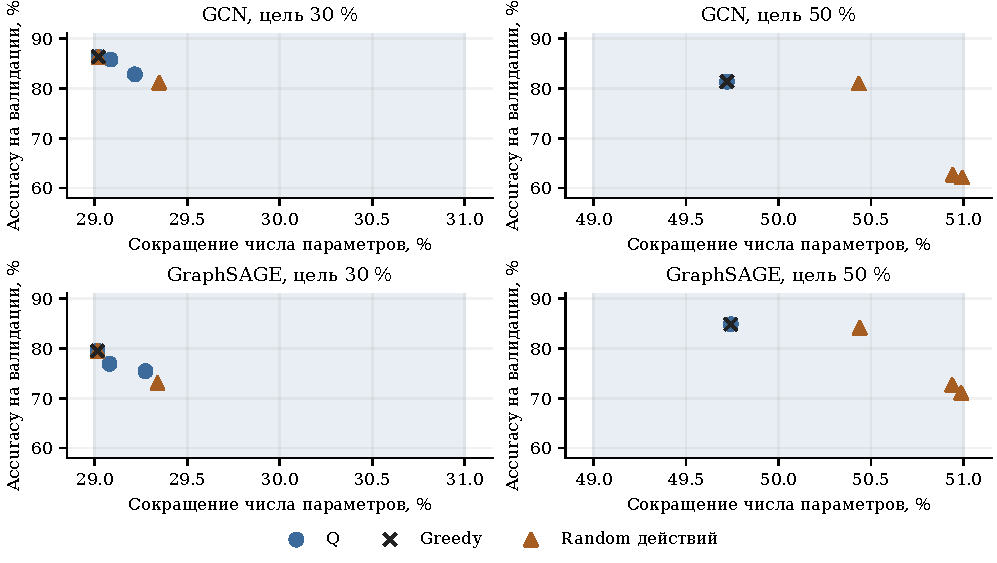
\includegraphics[width=\linewidth]{../figures/fig1_results.pdf}
\par\smallskip Рисунок 1. Фактическая компрессия и валидационная accuracy ограниченных стратегий. Точки соответствуют отдельным policy seed, вертикальные полосы — допустимым диапазонам цели. Все точки одной архитектуры используют один обученный checkpoint; совпадающие точки слегка различены маркерами, без изменения численных координат.
\end{figure}
Соблюдение одной полосы не означает точного совпадения компрессии. Например, при цели 50 \% Random сохраняет ширины 16$\times$7, 16$\times$8 или 16$\times$18, тогда как Q и Greedy сохраняют 16$\times$32. Поэтому полученные различия качества нельзя приписать только обучению с подкреплением. И при одинаковых ширинах разные последовательности текущего magnitude-удаления в общем случае способны сохранять разные каналы. Фильтр выравнивает допустимость структурных действий, но не фиксирует конечную архитектуру или подмножество параметров.

Цена поиска различается существенно. По сохранённым счётчикам при цели 30 \% constrained Q использовал 1035–1301 валидационную оценку для GCN и 1259–1312 для GraphSAGE, а Greedy — 38 и 34 соответственно. При цели 50 \% Q использовал 948–1130 и 1075–1216 оценок, Greedy — по 17. Средние времена поиска приведены в таблице 2. Они включают физические преобразования, копирование и валидацию в данном окружении. Эти значения позволяют оценить стоимость конкретной процедуры, но не являются временем инференса или оценкой чистой стоимости табличного обновления. Дополнительные эпизоды Q в этом наборе не дали лучшего среднего качества, чем дешёвый жадный контроль.

\subsection*{Геометрия ширин и вариативность масок}
Для обеих архитектур множество B при цели 30 \% содержит ровно 13 пар (23, b), b = 4…16, а при цели 50 \% — 26 пар (16, b), b = 7…32. Это следует из точного подсчёта параметров при F = 1433 и C = 7. Поскольку входная проекция содержит большую часть весов, уменьшение первой ширины сильнее влияет на число параметров, чем сопоставимое уменьшение второй. При узком допуске около 30 \% и максимально разрешённой первой ширине конечная вторая ширина вынужденно оказывается не более 16. Напротив, при 50 \% можно сохранить весь второй скрытый слой. Целевые множества не вложены друг в друга, а конкретные случайные маски между целями не являются последовательными стадиями одной траектории.

\par\medskip\noindent Таблица 3. Валидационная accuracy статического Random V2 по 20 маскам на условие\par
\begingroup\setlength{\tabcolsep}{2pt}\renewcommand{\arraystretch}{1.12}
\begin{longtable}{p{0.221\linewidth}p{0.111\linewidth}p{0.276\linewidth}p{0.332\linewidth}}
\toprule
Условие & Маски & Среднее $\pm$ SD, \% & Минимум–максимум, \%\\ \midrule\endhead
GCN 30 \% & 20 & 65,80 $\pm$ 16,58 & 22,37–88,54\\
GCN 50 \% & 20 & 71,19 $\pm$ 13,58 & 23,66–85,03\\
GraphSAGE 30 \% & 20 & 64,94 $\pm$ 19,94 & 11,46–85,95\\
GraphSAGE 50 \% & 20 & 72,13 $\pm$ 13,95 & 26,80–87,06\\
\bottomrule\end{longtable}\endgroup
\begin{figure}[htbp]\centering
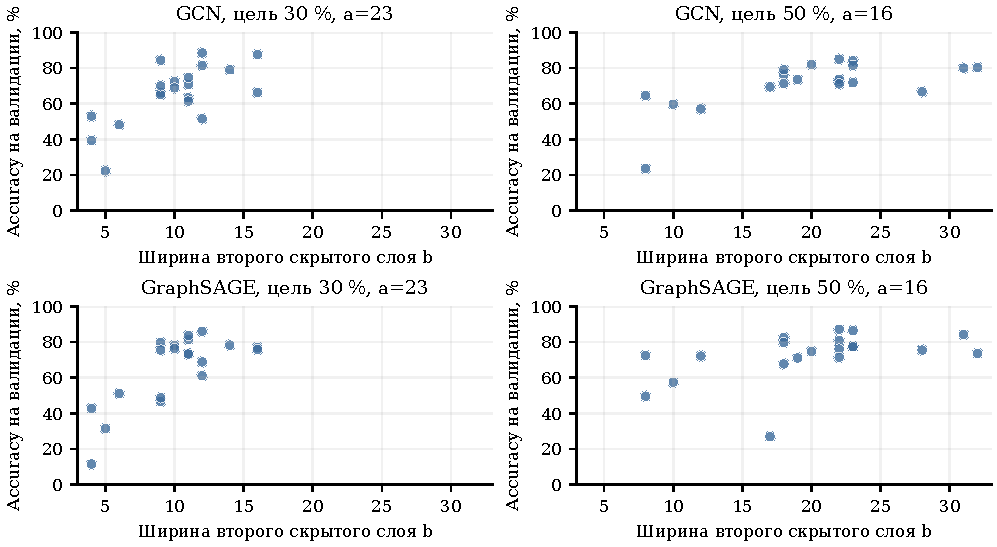
\includegraphics[width=\linewidth]{../figures/fig2_random.pdf}
\par\smallskip Рисунок 2. Валидационная accuracy 80 сохранённых случайных масок V2 в зависимости от второй скрытой ширины. В каждой панели первая ширина фиксирована целевым множеством. Вертикальный разброс при одинаковой второй ширине отражает различия конкретных сохраняемых каналов; линии между точками не проводятся.
\end{figure}
Как видно из таблицы 3, средняя accuracy при цели 50 \% в этой выборке выше, чем при 30 \%, у обеих моделей. Однако это не доказывает, что усиление компрессии улучшает качество: изменяется распределение допустимых архитектур и конкретных подмножеств. При фиксированных ширинах вариативность также велика. Для GCN 16$\times$8 две случайные маски различаются по accuracy на 40,85 п.п.; для GraphSAGE 23$\times$9 размах четырёх масок составляет 33,09 п.п. Следовательно, архитектурное объяснение не исчерпывает разброс. Точные причинные доли влияния ширин и идентичности каналов здесь не идентифицируются: группы несбалансированы, многие представлены одной маской. Максимальное качество отдельной маски не использовалось как результат baseline.

\subsection*{Парная воспроизводимость и границы измерений времени}
Во всех 34 парах локального исполнения и POLUS совпали последовательности финальных действий, обучающие действия, исходные идентификаторы сохраняемых каналов и тензоры итоговых checkpoint. Совпали исходная и финальная валидационные accuracy. Наибольшее расхождение macro-F1 равно 1,11$\times$10$^{-16}$. Из 24 непустых пар Q-таблиц 20 совпали точно, у остальных четырёх максимальное численное отличие составило 1,78$\times$10$^{-15}$ и не изменило выбранные действия. Пустые таблицы controls и probe не увеличивают число непустых сравнений.

Для двух фиксированных probe с конечными ширинами 27$\times$30 отдельно сохранены dense- и pruned-logits. Четыре соответствующие пары тензоров удовлетворяют rtol = 10$^{-5}$, atol = 10$^{-6}$; максимальное абсолютное расхождение равно 3,8147$\times$10$^{-6}$. Argmax совпадает на всех 2708 вершинах и на валидационной части. Сравнение предсказанных классов на всех вершинах не использует тестовые метки и не является оценкой test accuracy. Вывод относится к данному набору входов и политик, а не к универсальной побитовой воспроизводимости любых GNN.

Локальная среда: x86\_64, Python 3.12.9, Torch 2.2.2, PyG 2.6.1; одновременно работали два процесса по два потока. POLUS: POWER8 ppc64le, Python 3.10.22, Torch 2.0.1, PyG 2.4.0, один процесс с четырьмя потоками в выделенном задании. Поэтому отношения времени между платформами смешивают процессор, библиотеки, backend, число потоков и нагрузку. Они не интерпретируются как аппаратное ускорение.

\par\medskip\noindent Таблица 4. Сохранённые времена полного forward фиксированных probe в миллисекундах\par
\begingroup\setlength{\tabcolsep}{2pt}\renewcommand{\arraystretch}{1.12}
\begin{longtable}{p{0.166\linewidth}p{0.166\linewidth}p{0.304\linewidth}p{0.304\linewidth}}
\toprule
Платформа & Модель & Dense, мс & После удаления, мс\\ \midrule\endhead
Локально & GCN & 5,161 $\pm$ 0,447 & 5,449 $\pm$ 0,234\\
Локально & GraphSAGE & 30,202 $\pm$ 1,612 & 31,540 $\pm$ 5,336\\
POLUS & GCN & 7,514 $\pm$ 0,035 & 9,821 $\pm$ 0,065\\
POLUS & GraphSAGE & 19,442 $\pm$ 2,962 & 22,897 $\pm$ 2,684\\
\bottomrule\end{longtable}\endgroup
Для каждого измерения выполнены пять прогревов и 20 измеренных проходов; SD в таблице относится к проходам одного исполнения, а не к независимым timing-сессиям. Фиксированный прунинг уменьшил число параметров на 15,6863 \% для GCN и 15,6907 \% для GraphSAGE, но все четыре сохранённых средних времени после него оказались выше соответствующего dense. Это наблюдение не доказывает универсального замедления: число повторений и контроль нагрузки ограничены. Оно показывает, что параметрическая компрессия сама по себе не устанавливает ускорения в данном измерении.

\section*{Обсуждение и ограничения}
Основной результат состоит в разделении допустимости и выбора политики. Явная проверка достижимости устраняет один конкретный механизм неудачи — необратимый уход из множества состояний, из которых ещё можно попасть в диапазон за оставшиеся шаги. Отдельная коррекция STOP или инициализации Q такую геометрию не учитывает. При этом успешное попадание constrained Random показывает, что для соблюдения цели обучение не требуется. Сравнение с Greedy ограничивает интерпретацию роли Q: на имеющемся материале дополнительные эпизоды и таблица не сопровождаются лучшим средним качеством.

Награда не эквивалентна жёсткому двустороннему ограничению. Конечный штраф допускает отклонение при поиске, а оптимистичное нулевое значение неизвестного действия способно превышать уже выученные отрицательные оценки. Поэтому прохождение через диапазон и итоговое выполнение цели — разные события. Пороговая остановка уменьшает превышение, но не предотвращает дискретный перескок. В свою очередь, более высокая accuracy порогового варианта около 31,1 \% по сравнению с ограниченным вариантом около 29 \% не является сравнением при одинаковой компрессии: изменяются конечные ширины и сохраняемые каналы.

Выводы остаются пилотными по нескольким причинам. Исследован один граф, одно разбиение и один обученный checkpoint каждой архитектуры. Три policy seed оценивают локальную вариативность алгоритма; они не дают оценки чувствительности к обучению GNN. Детерминированные повторения Greedy имеют нулевой разброс качества по определению процедуры. Поэтому не рассчитывались p-values, доверительные интервалы превосходства или статистическая значимость разностей. Все результаты качества получены на валидации, участвующей в поиске, и могут быть оптимистичны относительно независимых данных. Ни один вывод не формулируется как test performance.

Состояние Q агрегирует разные подмножества каналов; вклад такой потери информации не изолирован отдельной абляцией. Кроме того, 100 эпизодов и $\lambda$ = 2 являются фиксированными настройками диагностического протокола, а не доказанно оптимальными гиперпараметрами. Отрицательный результат не означает невозможности успешного RL-прунинга с другой репрезентацией или бюджетом. Различия конечных ширин сохраняются даже внутри общего целевого диапазона, поэтому причинное преимущество именно обучаемой политики не идентифицировано.

Происхождение исходного графа восстановлено по записанным хешам исходных файлов и проверенной цепочке подготовки; хеш обработанного тензора, записанный непосредственно в момент исторического обучения не сохранялся. Зафиксированный сейчас тензор не выдаётся за такую историческую запись. Байтовые хеши checkpoint и разбиения, исходный порядок вершин и историческая сортировка рёбер сохранены. Это делает анализ прослеживаемым, но не устраняет указанное ограничение происхождения данных.

Наконец, параметры являются лишь одной составляющей затрат GNN. Агрегации на графе, перемещения данных и реализация вычислительных ядер могут определять фактическое время. Современные исследования эффективности GNN отдельно рассматривают ограничения доступа к памяти и организацию ядер \cite{r15}. Наши CPU-измерения не проверяют причинный вклад этих механизмов и не переносят результаты ускорения специализированных GPU-реализаций на текущие модели. Отсутствие новых экспериментов является границей настоящего анализа: изложенные ограничения определяют область выводов, а не скрытый план дополнения выборки.

\section*{Заключение}
Разработан и проверен на существующих результатах механизм ограничения локальных структурных действий по точной достижимости диапазона параметрической компрессии. Для поддерживаемых трёхслойных GCN и mean GraphSAGE он использует подсчёт всех весов и bias, множество конечных ширин и минимальное число допустимых удалений. При достижимой начальной цели и сохранении условий монотонного удаления механизм гарантирует принадлежность итоговой архитектуры целевому диапазону; гарантий качества или времени выполнения из этого не следует.

В пилоте Cora каждая из трёх ограниченных стратегий выполнила цель во всех 12 локальных оценках, тогда как отдельные изменения STOP, инициализации Q и разрешения равенств не обеспечили выполнение. Constrained Greedy имел не меньшую среднюю валидационную accuracy, чем constrained Q, во всех четырёх условиях при существенно меньшей стоимости поиска. Выбор ширин и конкретных каналов оказался существенен для интерпретации случайного baseline. Парные исполнения подтвердили совпадение политик и итоговых тензоров на двух CPU-платформах при малых различиях logits. На имеющихся данных обоснован явный контроль допустимости; преимущество Q-learning, независимое тестовое качество и ускорение инференса не установлены.

\section*{Доступность данных и программного обеспечения}
Код, компактные таблицы, протокол и сохранённые отчёты проверок опубликованы в репозитории проекта \cite{r16}. Для анализа зафиксирован head \texttt{34e8ca89\allowbreak 599b56ef\allowbreak 14bb4045\allowbreak 27b6a72d\allowbreak 6b26d403}; исполняемый исходный код V3 имеет SHA \texttt{7e2c760e\allowbreak 988b605e\allowbreak 305615de\allowbreak a147236e\allowbreak 8b0c59a3}. Исторический main \texttt{72293149\allowbreak d8fff186\allowbreak dd268789\allowbreak e7b8fea5\allowbreak 848c9360} не подменяет эту версию. Полные checkpoint, logits и трассы хранятся во внешнем архиве пользователя и индексированы в репозитории; их публичная доступность по постоянному адресу не подтверждена. Прилагаемые source\_manifest.csv и claim\_traceability.csv связывают таблицы и выводы с путями, коммитами и SHA256. Графики построены только по сохранённым CSV.

\section*{Благодарности и финансирование}
[ЗАПОЛНИТЬ АВТОРАМ: фактические источники поддержки, гранты, научный руководитель или консультант и основания для благодарности. При отсутствии финансирования указать это после подтверждения авторами.]

\section*{Вклад авторов и конфликт интересов}
[ЗАПОЛНИТЬ АВТОРАМ: вклад каждого автора в постановку, реализацию, выполнение ранее проведённых экспериментов, анализ и подготовку текста. Утвердить фактическое заявление о наличии или отсутствии конфликта интересов, оригинальности работы и отсутствии одновременной подачи.]

\section*{Использование средств искусственного интеллекта}
При подготовке данной версии рукописи использован Codex для анализа существующих файлов, проверки арифметики таблиц, подготовки текста, графиков и оформления. Новые научные эксперименты не выполнялись. [АВТОРАМ ПОДТВЕРДИТЬ И УТОЧНИТЬ: объём иной помощи ИИ в коде и предыдущих этапах исследования; ответственность за содержание и проверку ссылок несут авторы.]

\renewcommand{\refname}{Список литературы}\bibliographystyle{unsrtnat}\bibliography{references}
\section*{References}
\noindent 1. Kipf T. N., Welling M. Semi-Supervised Classification with Graph Convolutional Networks // International Conference on Learning Representations (ICLR). 2017. DOI (arXiv): 10.48550/arXiv.1609.02907. URL: \url{https://arxiv.org/abs/1609.02907} (accessed 27.10.2026).\par
\noindent 2. Hamilton W., Ying Z., Leskovec J. Inductive Representation Learning on Large Graphs // Advances in Neural Information Processing Systems. 2017. Vol. 30. DOI (arXiv): 10.48550/arXiv.1706.02216. URL: \url{https://papers.nips.cc/paper_files/paper/2017/hash/5dd9db5e033da9c6fb5ba83c7a7ebea9-Abstract.html} (accessed 27.10.2026).\par
\noindent 3. Liu Z., Li J., Shen Z., Huang G., Yan S., Zhang C. Learning Efficient Convolutional Networks through Network Slimming // Proceedings of the IEEE International Conference on Computer Vision (ICCV). 2017. P. 2736–2744. DOI (arXiv): 10.48550/arXiv.1708.06519. URL: \url{https://openaccess.thecvf.com/content_iccv_2017/html/Liu_Learning_Efficient_Convolutional_ICCV_2017_paper.html} (accessed 27.10.2026).\par
\noindent 4. Frankle J., Carbin M. The Lottery Ticket Hypothesis: Finding Sparse, Trainable Neural Networks // International Conference on Learning Representations (ICLR). 2019. DOI (arXiv): 10.48550/arXiv.1803.03635. URL: \url{https://arxiv.org/abs/1803.03635} (accessed 27.10.2026).\par
\noindent 5. Chen T., Sui Y., Chen X., Zhang A., Wang Z. A Unified Lottery Ticket Hypothesis for Graph Neural Networks // Proceedings of the 38th International Conference on Machine Learning. PMLR. 2021. Vol. 139. P. 1695–1706. URL: \url{https://proceedings.mlr.press/v139/chen21p.html} (accessed 27.10.2026).\par
\noindent 6. Zhang G., Yue Y., Wang K., Fang J., Sui Y., Wang K., Liang Y., Cheng D., Pan S., Chen T. Two Heads Are Better Than One: Boosting Graph Sparse Training via Semantic and Topological Awareness // Proceedings of the 41st International Conference on Machine Learning. PMLR. 2024. Vol. 235. P. 60197–60219. URL: \url{https://proceedings.mlr.press/v235/zhang24bx.html} (accessed 27.10.2026).\par
\noindent 7. Ma D., Chen J., Yang W., Gao S., Chen S. Pruning for GNNs: Lower Complexity with Comparable Expressiveness // Proceedings of the 42nd International Conference on Machine Learning. PMLR. 2025. Vol. 267. P. 41854–41889. URL: \url{https://proceedings.mlr.press/v267/ma25e.html} (accessed 27.10.2026).\par
\noindent 8. Lee N., Ajanthan T., Torr P. H. S. SNIP: Single-shot Network Pruning based on Connection Sensitivity // International Conference on Learning Representations (ICLR). 2019. DOI (arXiv): 10.48550/arXiv.1810.02340. URL: \url{https://arxiv.org/abs/1810.02340} (accessed 27.10.2026).\par
\noindent 9. Wang C., Zhang G., Grosse R. Picking Winning Tickets Before Training by Preserving Gradient Flow // International Conference on Learning Representations (ICLR). 2020. DOI (arXiv): 10.48550/arXiv.2002.07376. URL: \url{https://arxiv.org/abs/2002.07376} (accessed 27.10.2026).\par
\noindent 10. He Y., Lin J., Liu Z., Wang H., Li L.-J., Han S. AMC: AutoML for Model Compression and Acceleration on Mobile Devices // Computer Vision – ECCV 2018. Lecture Notes in Computer Science. 2018. Vol. 11211. P. 815–832. DOI: 10.1007/978-3-030-01234-2\_48. URL: \url{https://arxiv.org/abs/1802.03494} (accessed 27.10.2026).\par
\noindent 11. Liu Z., Sun M., Zhou T., Huang G., Darrell T. Rethinking the Value of Network Pruning // International Conference on Learning Representations (ICLR). 2019. DOI (arXiv): 10.48550/arXiv.1810.05270. URL: \url{https://arxiv.org/abs/1810.05270} (accessed 27.10.2026).\par
\noindent 12. Shchur O., Mumme M., Bojchevski A., Günnemann S. Pitfalls of Graph Neural Network Evaluation // Relational Representation Learning Workshop, NeurIPS. 2018. DOI (arXiv): 10.48550/arXiv.1811.05868. URL: \url{https://www.cs.cit.tum.de/en/daml/gnn-benchmark/} (accessed 27.10.2026).\par
\noindent 13. Watkins C. J. C. H., Dayan P. Q-learning // Machine Learning. 1992. Vol. 8. P. 279–292. DOI: 10.1007/BF00992698. URL: \url{https://link.springer.com/article/10.1007/BF00992698} (accessed 27.10.2026).\par
\noindent 14. Fey M., Lenssen J. E. Fast Graph Representation Learning with PyTorch Geometric // Representation Learning on Graphs and Manifolds Workshop, ICLR. 2019. DOI (arXiv): 10.48550/arXiv.1903.02428. URL: \url{https://arxiv.org/abs/1903.02428} (accessed 27.10.2026).\par
\noindent 15. Fomina D., Krasylnikov D., Boykov A., Dolgovyazov A., Zhdanovskiy V., Velikonivtsev F. On Efficient Scaling of GNNs via IO-Aware Layers Implementations // Proceedings of the 43rd International Conference on Machine Learning. PMLR. 2026. Vol. 306. P. 31329–31376. URL: \url{https://proceedings.mlr.press/v306/fomina26a.html} (accessed 27.10.2026).\par
\noindent 16. r1zons prunable\_gnn\_codex: source code and archived compact experimental results // GitHub repository. Version \texttt{34e8ca89\allowbreak 599b56ef\allowbreak 14bb4045\allowbreak 27b6a72d\allowbreak 6b26d403}. 2026. URL: \url{https://github.com/r1zons/prunable_gnn_codex/tree/34e8ca89599b56ef14bb404527b6a72d6b26d403} (accessed 27.10.2026).\par
\section*{Сведения об авторах}
[АВТОР 1: ФАМИЛИЯ ИМЯ ОТЧЕСТВО ПОЛНОСТЬЮ; учёная степень и звание или их отсутствие; организация; подразделение; должность или статус; город; страна; e-mail; автор для переписки; ORCID при наличии; другие идентификаторы при необходимости. Повторить для каждого соавтора.]

\section*{Information about the authors}
[AUTHOR 1: FULL NAME IN THE AUTHOR APPROVED ENGLISH SPELLING; degree and academic title or their absence; official affiliation; department; position or student status; city; country; email; corresponding author; ORCID if available. Repeat for each coauthor.]

\end{document}
